\chapter{环境配置与计算资源使用}

本章将主要介绍使用本地计算资源构建环境的方法。同学们在进行实验时,原则上使用本章任意一节的知识即可完成所有实验,但推荐同学们掌握多种方法。相信大多数同学在课前已经掌握了\S\ref{sec:local-env}节中本地环境的配置方法,而\S\ref{sec:env-setup-docker}节中介绍的Docker的使用则不为大多数同学所熟知,因此推荐同学掌握Docker的使用方法,Docker在今后的科研和开发中也有望帮助同学们事半功倍。

\section{使用本地环境与GPU}\label{sec:local-env}

使用本地计算资源可以不收网络链接状况约束,随时随地调试程序,对于简单的项目,本地调试也可能更省时间。

本节以助教所使用的计算机为例,展示环境配置过程。助教使用的计算机系统与配置为:
\begin{itemize}
    \item 系统:windows10专业教育版;22H2
    \item 处理器:Intel(R) Core(TM) i7-8700 CPU 
    \item 内存:16GB
    \item 显卡:NVIDIA GeForce RTX 2060
    \item 编辑器:Visual Studio Code
\end{itemize}

\subsection{安装CUDA工具箱}

对于包含英伟达显卡的计算机,我们推荐首先安装CUDA工具包以使用GPU加速计算。

\textcolor{red}{\emph{注意,仅包含英伟达GPU的计算机需要安装CUDA工具箱以使用GPU加速计算。使用核显或AMD显卡的计算机再后续步骤中使用CPU计算即可。}}

GPU型号、CUDA工具包、PyTorch版本相互关联。因此需要一起规划好。

首先查看自己的显卡的算力\url{https://developer.nvidia.com/zh-cn/cuda-gpus}:
查看得到我的显卡的2060的算力为7.5,图\ref{fig:nvidia-rtx-2060-capability}。

\begin{figure}[htbp]
    \centering
    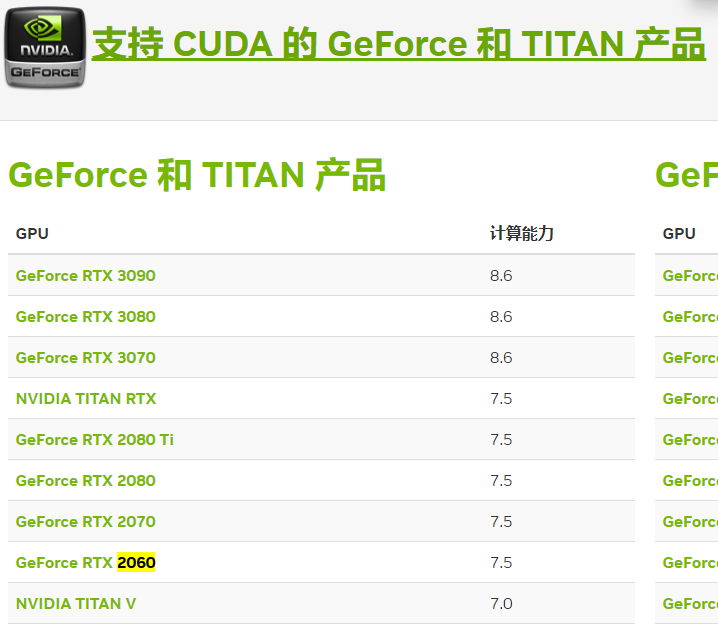
\includegraphics[width=0.7\textwidth]{figures/nvidia-rtx-2060-capability.png}
    \caption{fig:nvidia-rtx-2060-capability}
    \label{fig:nvidia-rtx-2060-capability}
\end{figure}

然后根据算力查看支持该算力的CUDA版本\url{https://en.wikipedia.org/wiki/CUDA}:
查看得到支持我显卡的CUDA版本为$\geq$10.0,图\ref{fig:corresponding-cuda-version}。
\begin{figure}[htbp]
    \centering
    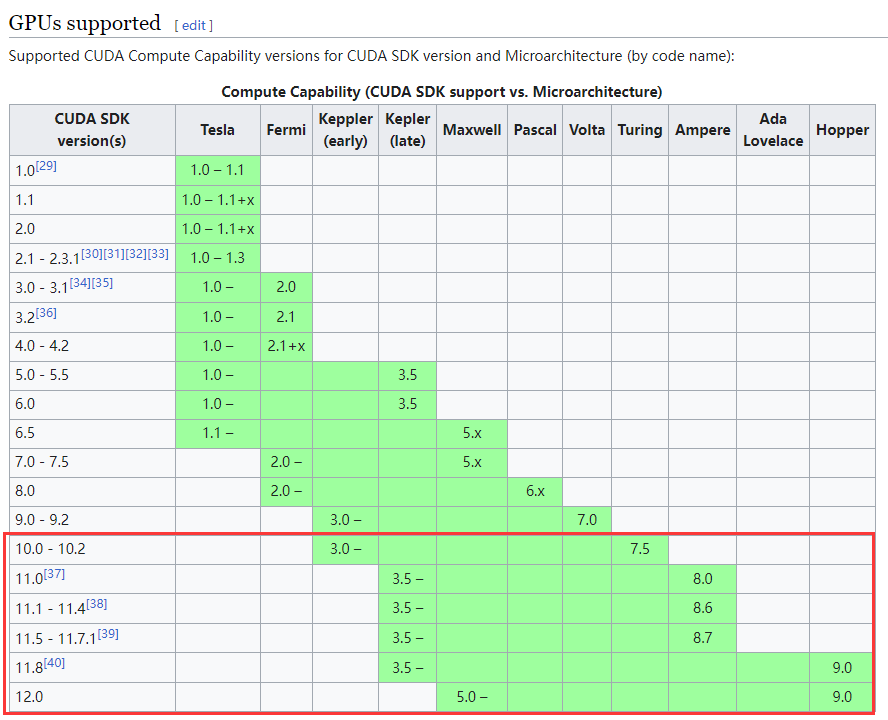
\includegraphics[width=0.9\textwidth]{figures/corresponding-cuda-version.png}
    \caption{fig:corresponding-cuda-version}
    \label{fig:corresponding-cuda-version}
\end{figure}

同时CUDA对显卡驱动的最低版本也提出了要求\url{https://docs.nvidia.com/cuda/cuda-toolkit-release-notes/index.html},但显卡驱动对CUDA向下兼容,因此一般安装了最近发布的显卡驱动版本即可,无需与CUDA版本特别对应。




最后要注意,PyTorch并不一定支持最新的CUDA版本,因此安装前再去PyTorch上看一眼PyTorch支持哪些CUDA版本,图\ref{fig:cuda-version-constrained-by-pytorch}:\url{https://pytorch.org/get-started/locally/}
\begin{figure}[htbp]
    \centering
    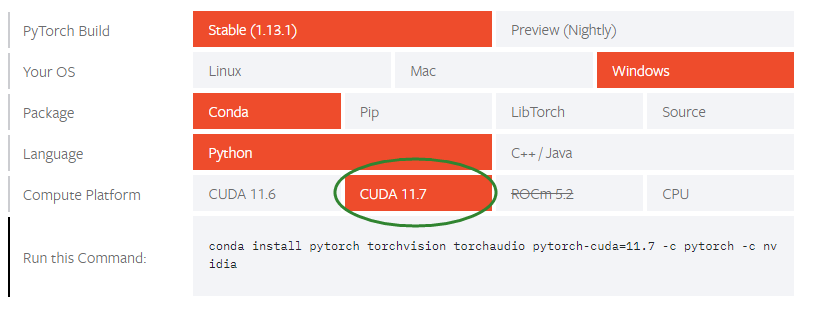
\includegraphics[width=0.8\textwidth]{figures/cuda-version-constrained-by-pytorch.png}
    \caption{fig:cuda-version-constrained-by-pytorch}
    \label{fig:cuda-version-constrained-by-pytorch}
\end{figure}

我们发现PyTorch最高支持到CUDA 11.7,满足显卡算力对CUDA版本$\geq$10.0的要求,因此我们可以选择安装CUDA 11.7。

选择对应版本CUDA安装包并下载安装, 安装过程略,图\ref{fig:select-cuda-version}:
\url{https://developer.nvidia.com/cuda-toolkit-archive}

\begin{figure}[htbp]
	\centering
	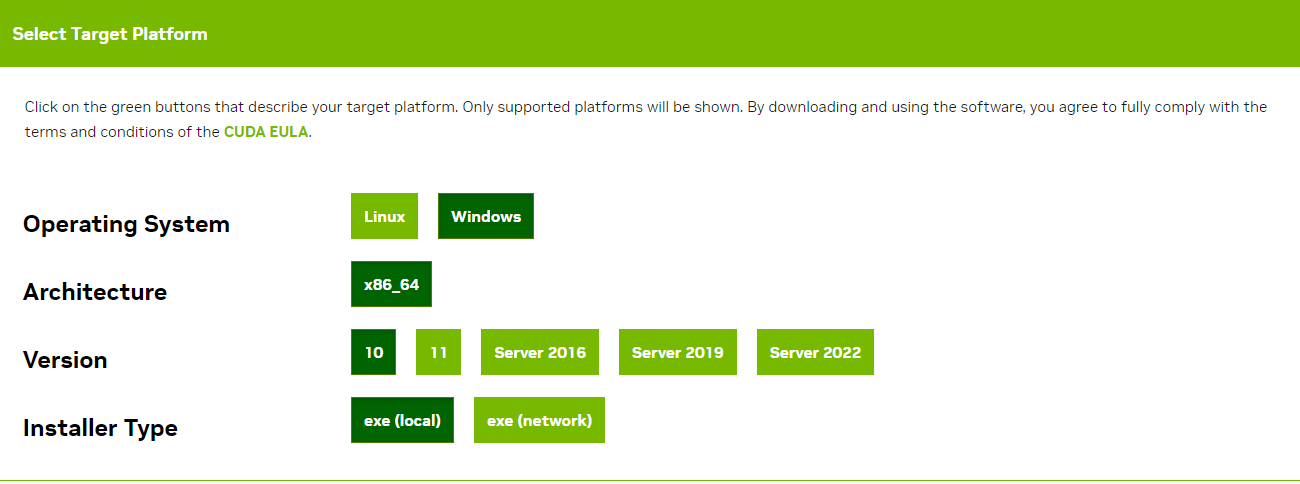
\includegraphics[width=0.8\textwidth]{figures/select-cuda-version.png}
	\caption{fig:select-cuda-version}
	\label{fig:select-cuda-version}
\end{figure}

在这一步完成后,我们打开终端输入\graylstinline{nvcc -V}以及\graylstinline{nvidia-smi}应当分别能看到图\ref{fig:nvcc-v-install-success}和图\ref{fig:nvidia-smi-install-success}类似的输出,这说明我们安装完成。

\begin{figure}[htbp]
	\centering
	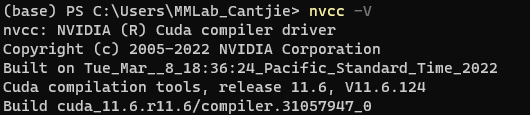
\includegraphics[width=0.7\textwidth]{figures/nvcc-v-install-success.png}
	\caption{caption:nvcc-v-install-success}
	\label{fig:nvcc-v-install-success}
\end{figure}

\begin{figure}[htbp]
	\centering
	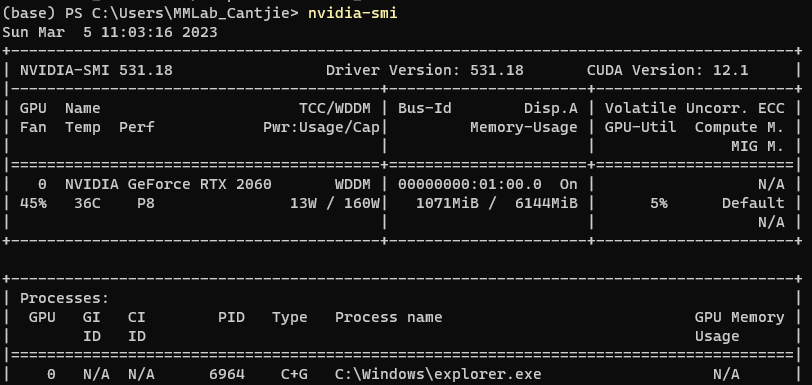
\includegraphics[width=0.8\textwidth]{figures/nvidia-smi-install-success.png}
	\caption{caption:nvidia-smi-install-success}
	\label{fig:nvidia-smi-install-success}
\end{figure}

\subsection{安装Anaconda}

我们可能同时有多个项目或作业在处理,而不同的项目或作业可能使用了不同python版本、不同的工具包等,为了避免冲突,我们通常会为每一个项目或作业指定一个虚拟环境,以使得各个环境之间互不干扰。为此,我们Anaconda以创建并管理虚拟环境。

安装过程参考官网文档即可:
\url{https://docs.anaconda.com/anaconda/install/windows/}

安装完成后启动终端,输入\graylstinline{conda -V},如正确显示conda版本则说明安装成功。
\begin{figure}[htbp]
	\centering
	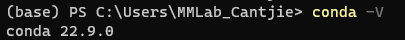
\includegraphics[width=0.7\textwidth]{figures/conda-install-success.png}
	\caption{caption:conda-install-success}
	\label{fig:conda-install-success}
\end{figure}

\subsection{创建虚拟环境并安装PyTorch} \label{subsec:local-env-create}

安装完成conda后,我们新建一个预装了Python的、用来完成本门课程的虚拟环境。

需要注意的是,PyTorch和Python版本也需要对应,在\url{https://github.com/pytorch/vision#installation}中,我们发现torch 1.13要求python 介于3.7.2和3.10之间。

\begin{figure}[htbp]
	\centering
	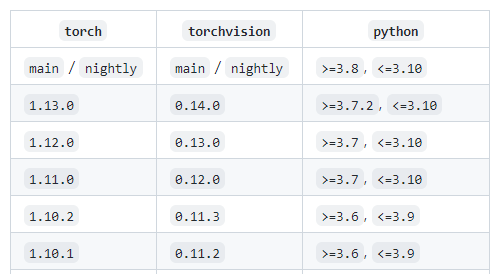
\includegraphics[width=0.7\textwidth]{figures/pytorch-python-version-compability.png}
	\caption{caption:pytorch-python-version-compability}
	\label{fig:pytorch-python-version-compability}
\end{figure}

打开终端,输入下面命令以利用conda新建环境,
\begin{lstlisting}
    $ conda create --name <envname> python=3.9
\end{lstlisting}
将其中<envname>改成自定义的环境名称,如助教自己选择的distributedml。

新建完成后,通过\graylstinline{conda activate <envname>}进入环境。在pytorch官网安装页面\url{https://pytorch.org/get-started/locally/}选择对应的pytorch版本、系统版本等,复制给出的命令并运行。

\begin{figure}[htbp]
	\centering
	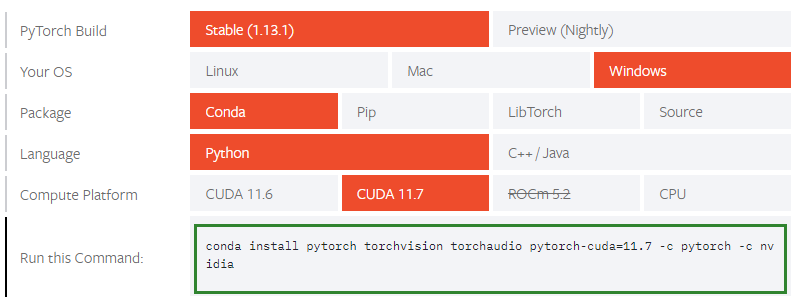
\includegraphics[width=1\textwidth]{figures/pytorch-install-command.png}
	\caption{caption:pytorch-install-command}
	\label{fig:pytorch-install-command}
\end{figure}

安装完成后,进入Python就可以\graylstinline{import torch}了,如图\ref{fig:pytorch-install-success}.

\begin{figure}[htbp]
	\centering
	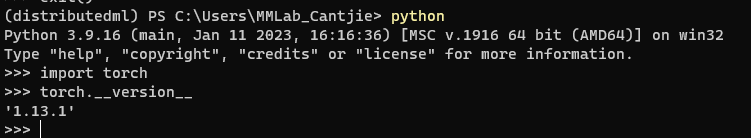
\includegraphics[width=0.7\textwidth]{figures/pytorch-install-success.png}
	\caption{caption:pytorch-install-success}
	\label{fig:pytorch-install-success}
\end{figure}

\subsection{安装其他包}

如果我们还想要安装其他包,比如同学们画图常用的matplotlib包,该怎么办呢?在\graylstinline{conda activate <envname>}进入环境后,直接通过\graylstinline{conda install matplotlib}就可以了。

% \subsection{使用VSCode编辑python文件}

% 以实验一为例,VSCode安装Python插件后,


\section{使用虚拟环境与本地GPU}\label{sec:env-setup-docker}

上面的本地环境配置不可为不复杂,CUDA、显卡型号、显卡驱动、PyTorch、Python等版本需要手动一一对应起来安装。那有没有什么更简单的利用本机GPU计算资源的方法呢?

在这一节,我们介绍直接利用Docker镜像搭配环境的方法。

\subsection{安装并配置Docker引擎}

首先在官网下载安装包\url{https://docs.docker.com/desktop/install/windows-install/},安装过程略。

在安装完成后启动Docker Desktop,在windows下,很可能会报错(具体内容是啥助教忘了截图了),一般错误的原因是缺少wsl2和hyper-v。

为了启用hyper-v,在控制面板中按照图\ref{fig:turn-on-hyper-v}中的操作选中Hyper-V并确定。
\begin{figure}[htbp]
	\centering
	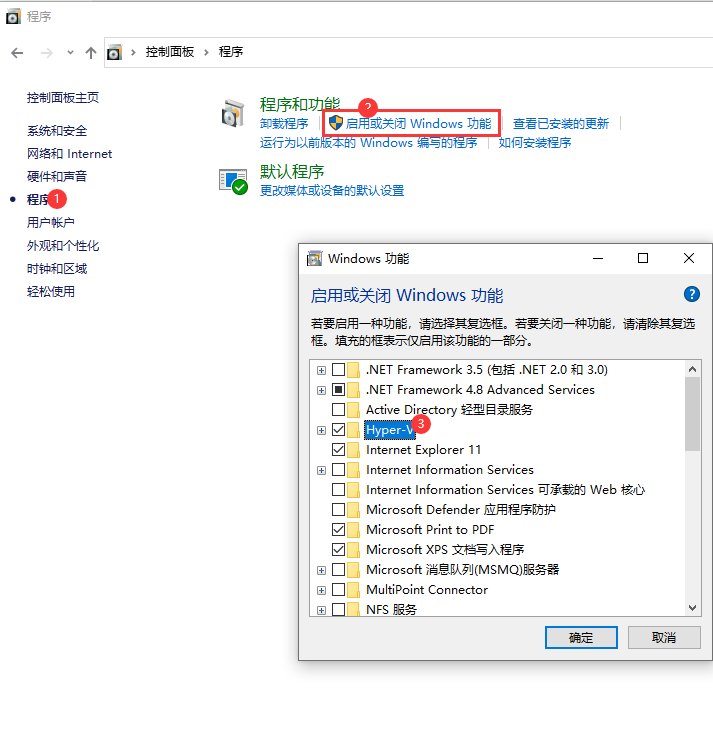
\includegraphics[width=1\textwidth]{figures/turn-on-hyper-v.png}
	\caption{caption:turn-on-hyper-v}
	\label{fig:turn-on-hyper-v}
\end{figure}

为了启用wsl2,参考\url{https://learn.microsoft.com/en-us/windows/wsl/install},在终端下输入\graylstinline{wsl --install}等待安装完成即可。

\begin{figure}[htbp]
	\centering
	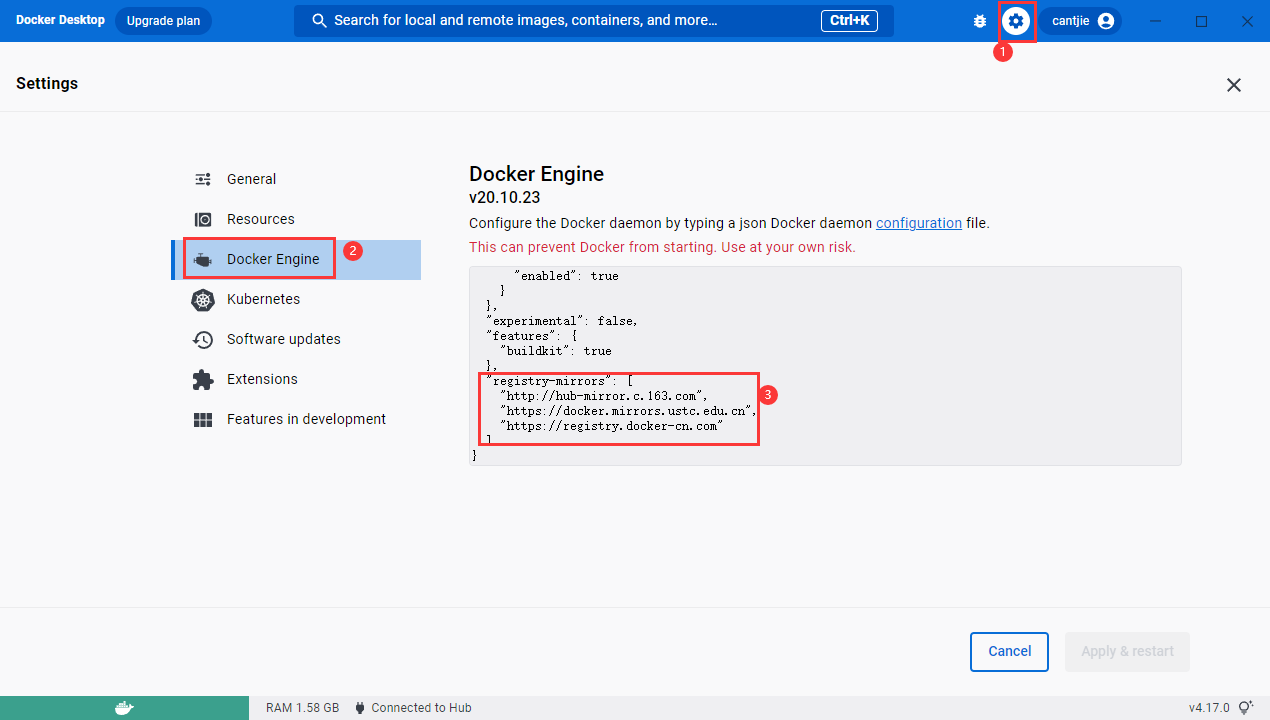
\includegraphics[width=0.9\textwidth]{figures/docker-mirrors-setting.png}
	\caption{caption:docker-mirrors-setting}
	\label{fig:docker-mirrors-setting}
\end{figure}

安装完成后启动Docker Desktop,为了加速下载,可以按照图\ref{fig:docker-mirrors-setting}所示方法为Docker指定国内镜像服务器,即在原本的配置中加入如下内容。
\begin{lstlisting}
    "registry-mirrors": [
        "http://hub-mirror.c.163.com",
        "https://docker.mirrors.ustc.edu.cn",
        "https://registry.docker-cn.com"
    ]
\end{lstlisting}

启动终端,输入\graylstinline{docker --version},如图\ref{fig:docker-install-success},正常返回Docker版本就说明安装成功了。
\begin{figure}[htbp]
	\centering
	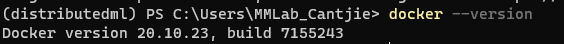
\includegraphics[width=0.7\textwidth]{figures/docker-install-success.png}
	\caption{caption:docker-install-success}
	\label{fig:docker-install-success}
\end{figure}


\subsection{搜索并下载PyTorch镜像}

Dockerhub是一个共享镜像的平台\url{https://hub.docker.com/}。所谓镜像,类似于一个操作系统的iso文件:我们拿到iso文件后可以创建使用该操作系统的虚拟机;而当我们拿到镜像后,也可以利用该镜像创造一个使用该镜像的容器,即容器是一个镜像的实例。

因此,如果有人在某个容器中把CUDA、PyTorch、Python等环境都配置好,并打包成镜像共享给我们,我们就可以免去复杂的安装过程,从而直接使用镜像生成容器,在容器中直接运行我们所写的脚本。

在DockerHub中,我们搜索\graylstinline{pytorch/pytorch},可以找到对应的这个镜像\url{https://hub.docker.com/r/pytorch/pytorch}。点击网页中的Tags标签页,我们可以从图\ref{fig:pytorch-image-tags-web}看到这个镜像就是已经把PyTorch和CUDA安装好了的,我们直接使用这个镜像就好啦!

\begin{figure}[htbp]
	\centering
	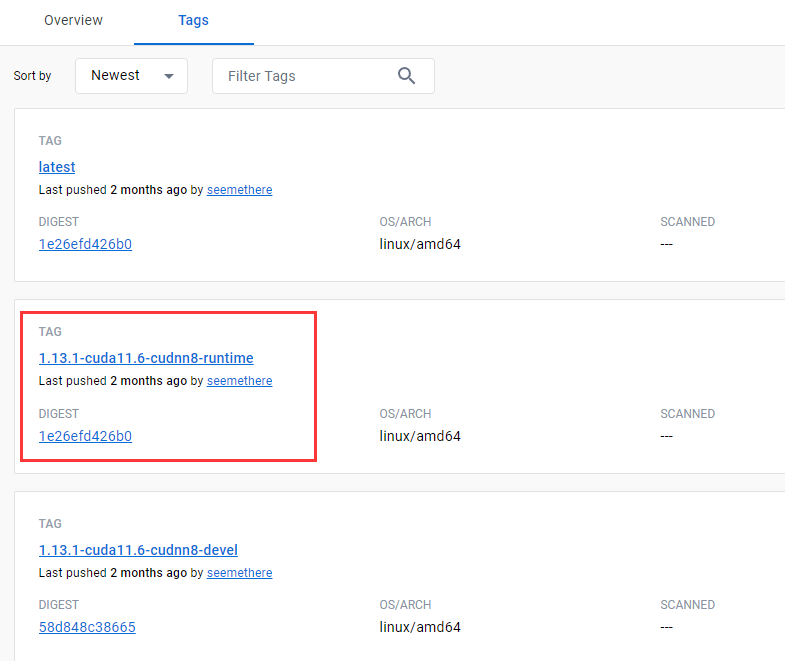
\includegraphics[width=0.7\textwidth]{figures/pytorch-image-tags-web.png}
	\caption{caption:pytorch-image-tags-web}
	\label{fig:pytorch-image-tags-web}
\end{figure}

下载这个镜像前,还需要登录的。首先去注册个账号,然后打开终端,输入\graylstinline{docker login}登录。

然后就可以通过这条命令下载这个镜像了:

\begin{lstlisting}
    $ docker pull pytorch/pytorch:1.13.1-cuda11.6-cudnn8-runtime
\end{lstlisting}


这个镜像比较大,下载需要一点时间。完成后,我们再输入\graylstinline{docker image list}就可以看到这个镜像了,见图\ref{fig:docker-image-list-pytorch}。
\begin{figure}[htbp]
	\centering
	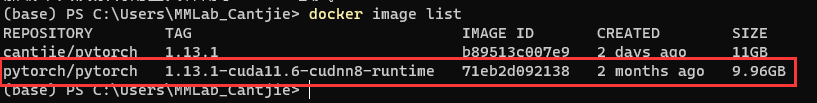
\includegraphics[width=0.9\textwidth]{figures/docker-image-list-pytorch.png}
	\caption{caption:docker-image-list-pytorch}
	\label{fig:docker-image-list-pytorch}
\end{figure}

\subsection{启动容器}

下载完镜像,我们该通过这个镜像启动一个容器了,我们需要到容器里看看这个容器里面是不是有我们需要的环境。

打开终端,输入
\begin{lstlisting}
    $ docker run -it pytorch/pytorch:1.13.1-cuda11.6-cudnn8-runtime
\end{lstlisting}
我们发现我们进入了一个linux系统,进去运行一下\graylstinline{nvidia-smi}试试,诶,怎么command not found,看不到显卡。这是因为容器启动时没有给他指定GPU。我们输入\graylstinline{exit},然后加上GPU参数再试一下
\begin{lstlisting}
    $ docker run --gpus all -it pytorch/pytorch:1.13.1-cuda11.6-cudnn8-runtime 
\end{lstlisting}

进入容器后,我们输入\graylstinline{nvidia-smi}等命令,查看运行结果,如图\ref{fig:docker-pytorch-container-env-check}所示,发现正是我们所需要的环境。
\begin{figure}[htbp]
	\centering
	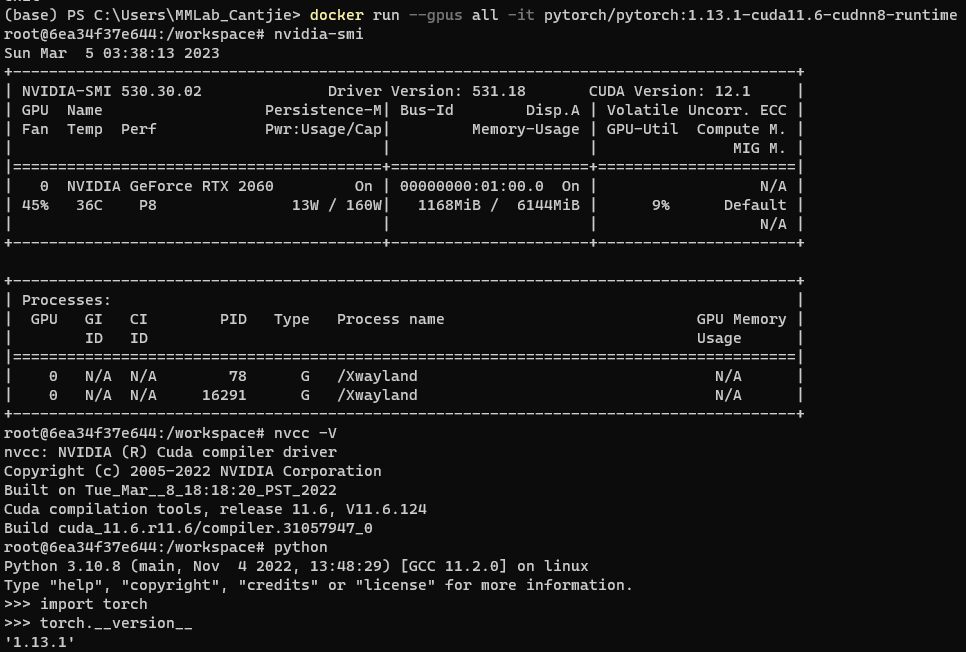
\includegraphics[width=1\textwidth]{figures/docker-pytorch-container-env-check.png}
	\caption{caption:docker-pytorch-container-env-check}
	\label{fig:docker-pytorch-container-env-check}
\end{figure}


\subsection{安装新包后重新打包成镜像}\label{subsec:container-to-image}

但是,也有一些包在默认的镜像里是没有的,万一我们需要这些包,比如matplotlib包,难道我们要每次启动新的容器之后都手动通过\graylstinline{conda install}安装一下么?不用的,我们安装一次之后,将这个容器重新打包成一个新的镜像就好了!我们之后再用,就用新的镜像了。

\begin{figure}[htbp]
	\centering
	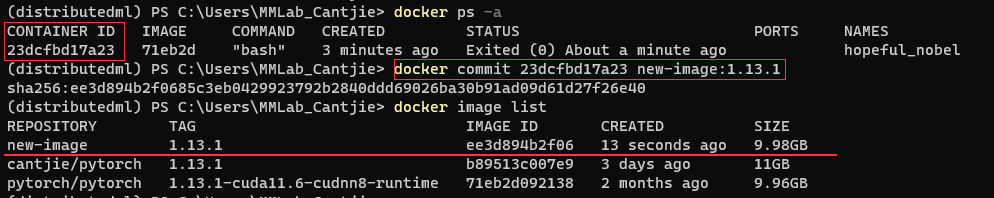
\includegraphics[width=1\textwidth]{figures/docker-commit-new-image.png}
	\caption{caption:docker-commit-new-image}
	\label{fig:docker-commit-new-image}
\end{figure}

在刚才启动的容器里,我们输入\graylstinline{conda install matplotlib},安装完成后,输入\graylstinline{exit}退出容器。回到windows下的命令行,输入\graylstinline{docker ps -a}查看所有容器,如图\ref{fig:docker-commit-new-image}所示,我们发现刚刚安装了matplotlib的容器的id为\graylstinline{23dcfbd17a23}。接下来,我们运行
\begin{lstlisting}
	$ # docker commit <containerID> <new-image-name>:<tags>
	$ docker commit 23dcfbd17a23 new-image:1.13.1
\end{lstlisting}
便将容器打包成了一个镜像。输入\graylstinline{docker image list},便可以看到我们新建的容器了。

以后就都可以用这个新镜像了,可是如何使用这个环境呢,我们留到完成具体实验内容的时候再来讲。

\subsection{限制Docker内存占用(可选)}

由于docker占用内存很大,对于内存不足的电脑可能造成卡顿现象,可以通过修改配置文件限制其内存占用。

修改C:\textbackslash users\textbackslash<username>\textbackslash .wslconfig 

\begin{lstlisting}
[wsl2]
memory=6GB
swap=6GB
swapfile=E:\\wsl-swap.vhdx
\end{lstlisting}





% \section{使用深研院计算资源}\label{sec:env-setup-sigs-resources}

% % \textcolor{red}{\emph{注意,在该平台启动的开发环境需要首先手动调整一下DNS服务器,即在\graylstinline{/etc/resolv.conf}最上方添加一行“\graylstinline{nameserver 114.114.114.114}”即可。}}

% 助教会为同学们下发用户名和密码。使用自己的账户信息登录网址:\url{http://10.103.9.27:30000/}(或使用助教的域名\url{http://sigs-gpu.cantjie.com:30000})。注意,账号可能是共享的,请同学们格外留意\emph{在创建开发环境时不要占用账号下的全部资源。}

% \subsection{创建开发环境}

% 登录系统后,我们需要创建一个开发环境。如图\ref{fig:sigs-platform-dev-env-before-create}所示,首先在左侧边栏选择AI分区->开发环境,然后点击创建。

% \begin{figure}[htbp]
% 	\centering
% 	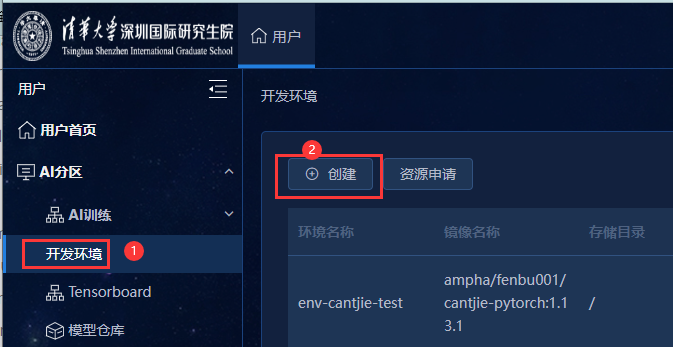
\includegraphics[width=0.7\textwidth]{figures/sigs-platform-dev-env-before-create.png}
% 	\caption{caption:sigs-platform-dev-env-before-create}
% 	\label{fig:sigs-platform-dev-env-before-create}
% \end{figure}

% \begin{figure}[htbp]
% 	\centering
% 	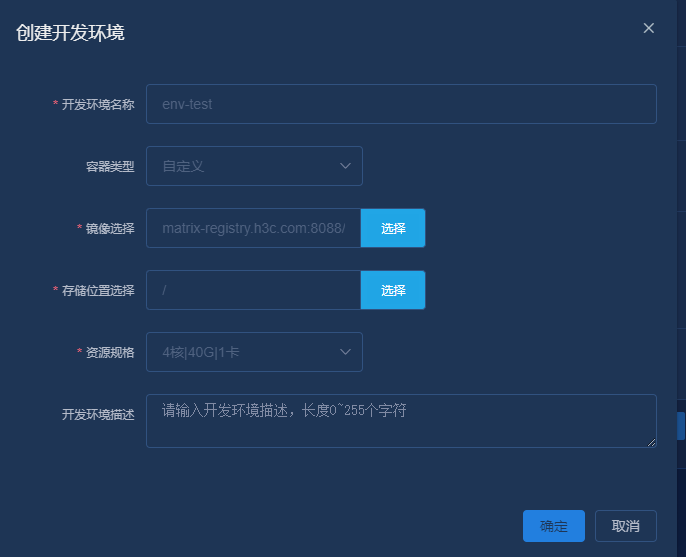
\includegraphics[width=0.6\textwidth]{figures/sigs-platform-dev-env-create.png}
% 	\caption{caption:sigs-platform-dev-env-create}
% 	\label{fig:sigs-platform-dev-env-create}
% \end{figure}
% 在弹出的窗口图\ref{fig:sigs-platform-dev-env-create}中,设置环境名称、镜像、储存位置、资源规格等信息。其中,当与小组同学共享账号时,请不要直接选择默认的资源规格,请通过自定义,限制环境所需的CPU核心数量、储存空间大小和显卡数量(譬如六人共享账号时,推荐每个人都将资源设置为最大可用资源的六分之一)。对于我们的实验,系统自带的镜像已基本可以满足需求,因此在镜像选择中,按图\ref{fig:sigs-platform-dev-env-image-selection}所示选择superadmin/pytorch:1.12.0-cuda11.3-cudnn8-runtime-2即可(注意末尾的-2,带-2的版本为本学期初根据课程需求定制的版本,不带-2的版本使用ssh连接进入后会找不到合适环境。)。


% \begin{figure}[htbp]
% 	\centering
% 	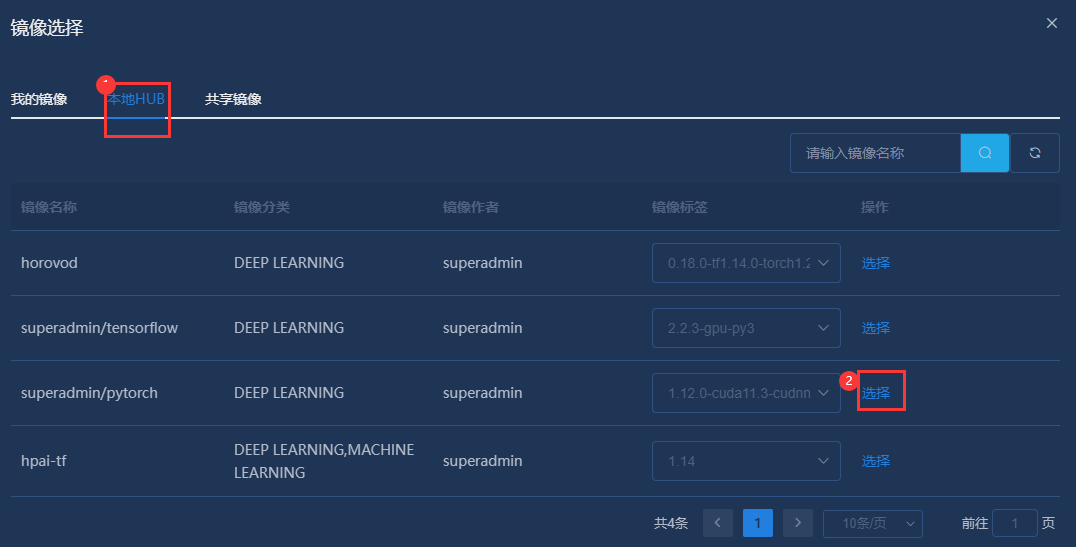
\includegraphics[width=0.8\textwidth]{figures/sigs-platform-dev-env-image-selection.png}
% 	\caption{caption:sigs-platform-dev-env-image-selection}
% 	\label{fig:sigs-platform-dev-env-image-selection}
% \end{figure}

% 创建时指定的储存路径会挂载到环境的\graylstinline{/private}目录下。

% \subsection{安装其他软件或包}

% 新建完成后,点击启动,等待镜像状态变为运行中,访问方式一栏会出现SSH、远程桌面和VNC三种连接方式,操作一栏的打开按钮也会有灰变蓝。

% 当我们需要使用镜像中尚未安装的工具或包时,可以通过访问方式提供的三种方式安装,譬如,在本地使用ssh连接服务器后,运行\graylstinline{conda install matplotlib}或\graylstinline{apt install git}等;也可通过点击打开按钮,在弹出页面中进入终端并安装,见图\ref{fig:sigs-platform-env-install-packages-via-web}。

% \begin{figure}[htbp]
% 	\centering
% 	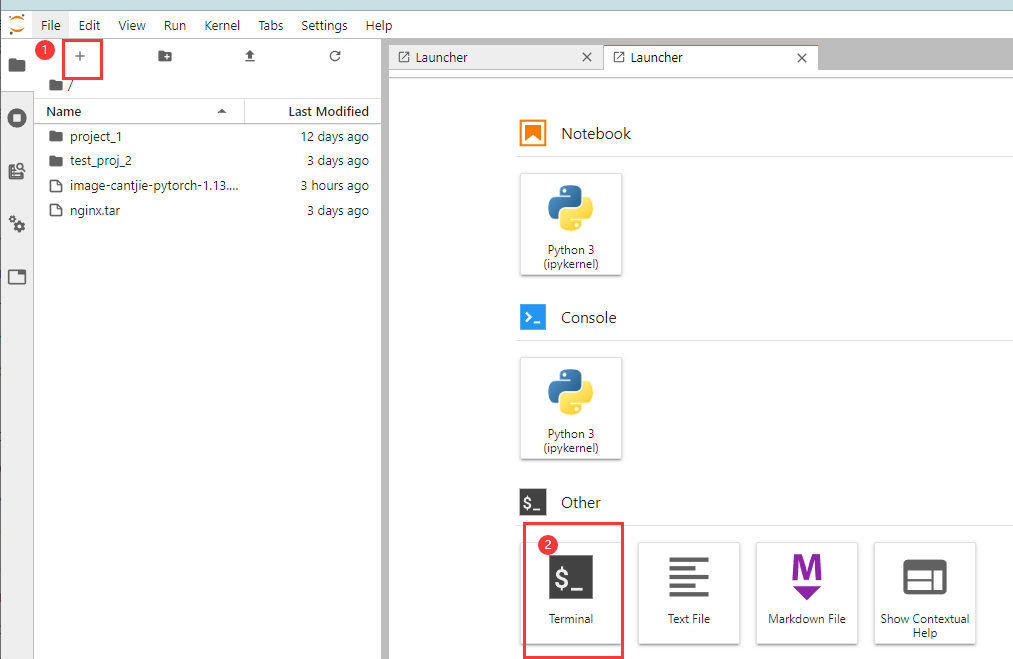
\includegraphics[width=0.9\textwidth]{figures/sigs-platform-env-install-packages-via-web.png}
% 	\caption{caption:sigs-platform-env-install-packages-via-web}
% 	\label{fig:sigs-platform-env-install-packages-via-web}
% \end{figure}




% \subsection{创建镜像环境}

% \textcolor{red}{\emph{注意,截止本指导书书发布时,由于平台缺乏技术文档,个人制作的镜像可能无法让容器正常启动。该小节仍有待完善。}}

% \textcolor{red}{\emph{注意,该平台为x86架构,arm平台上创建的镜像无法运行在该平台}}

% 镜像创建方法可参考\S\ref{subsec:container-to-image}。


% 在本地创建镜像后,使用\graylstinline{docker save -o filename.tar imagename:tag}\footnote{注意,此处不可使用sha256格式的imageID代替<imagename>:<tag>的格式,不然平台可能无法正确处理该镜像}命令导出镜像文件,然后上传至文件管理->我的文件栏目下(图\ref{fig:sigs-platform-upload-file})。然后在镜像服务->我的镜像中创建镜像(图\ref{fig:sigs-platform-create-custom-image})。

% \begin{figure}[htbp]
% 	\centering
% 	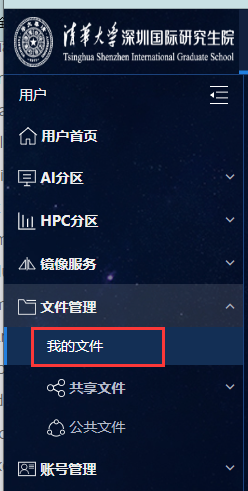
\includegraphics[width=0.25\textwidth]{figures/sigs-platform-upload-file.png}
% 	\caption{caption:sigs-platform-upload-file}
% 	\label{fig:sigs-platform-upload-file}
% \end{figure}


% \begin{figure}[htbp]
% 	\centering
% 	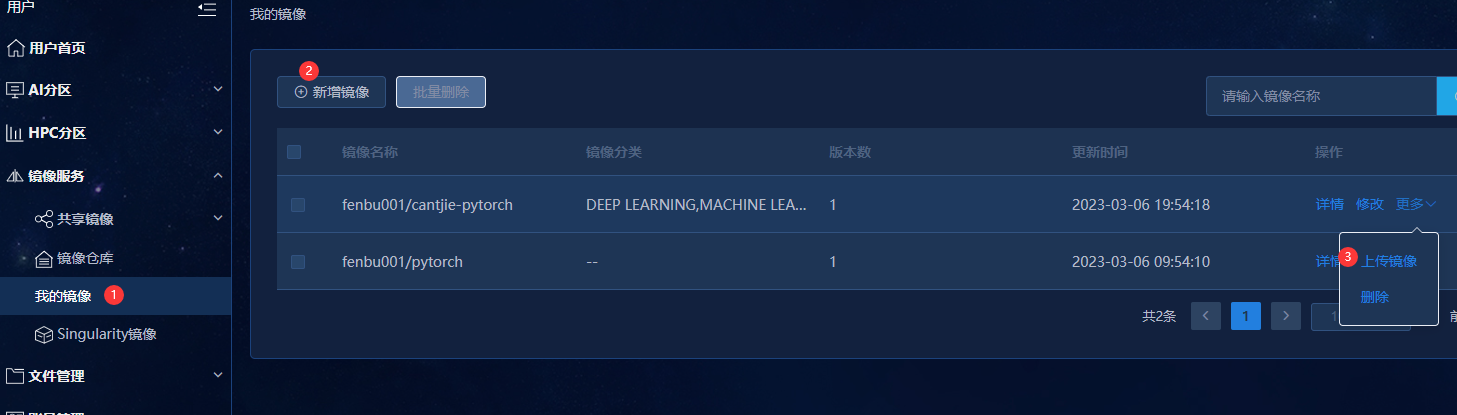
\includegraphics[width=1\textwidth]{figures/sigs-platform-create-custom-image.png}
% 	\caption{caption:sigs-platform-create-custom-image}
% 	\label{fig:sigs-platform-create-custom-image}
% \end{figure}



